\documentclass[conference]{IEEEtran}
\usepackage{amsmath,amssymb,amsthm}
\usepackage[T1]{fontenc}
\usepackage{listings}
\usepackage{booktabs}
\usepackage{graphicx}
\usepackage{algorithm}
\usepackage{algpseudocode}
\usepackage{hyperref}
\hypersetup{hidelinks}
\newtheorem{theorem}{Theorem}
\newtheorem{lemma}{Lemma}
\newcommand{\Oh}{\mathcal{O}}
\title{Exact Subset Sum: Reproducible Baselines, Measurements,\\
and a Bounded-Magnitude Result}
\author{\IEEEauthorblockN{Reproducible Research Note}}
\begin{document}
\maketitle
\begin{abstract}
We study the exact decision problem: given integers $a_1,\dots,a_n,b$,
is there $x\in\{0,1\}^n$ with $\sum_i a_i x_i=b$? Whether the classical
$\Oh^*(2^{n/2})$ worst-case barrier can be improved to $\Oh^*(2^{n/3})$
is a long-standing open question; we do not resolve it. We instead collect
deterministic witness-producing solvers---sorted meet-in-the-middle, a signed
dynamic program, and Schroeppel--Shamir---give mathematical correctness and
runtime arguments, formalize the correctness layer in Lean~4, and measure all
three on infeasible instances. The measurements reproduce the predicted
$\Oh^*(2^{n/2})$ time and confirm the $\Oh^*(2^{n/4})$ peak-memory advantage of
Schroeppel--Shamir over meet-in-the-middle. A signed dynamic program solves
every instance with magnitude sum $W=\sum_i|a_i|\le 2^{\lfloor n/3\rfloor}$ in
$\Oh^*(2^{n/3})$ time; this is the textbook pseudopolynomial bound and not a
general algorithm. The open bound, the restricted theorem, the proofs, and the
finite measurements are kept strictly distinct.
\end{abstract}
\begin{IEEEkeywords}
subset sum, exact exponential algorithms, meet-in-the-middle, Schroeppel--Shamir,
formal verification, reproducibility
\end{IEEEkeywords}

\section{Problem and Scope}
Given $a_1,\dots,a_n,b\in\mathbb{Z}$, determine whether
\begin{equation}\label{eq:problem}
\exists x\in\{0,1\}^n:\quad\sum_{i=1}^{n}a_i x_i=b.
\end{equation}
The empty subset is permitted. Equal-valued entries are distinct occurrences,
each available at most once. Negative entries and targets are permitted. This
is the equality-decision form of 0--1 knapsack.

A classical result decides \eqref{eq:problem} on every input in
$\Oh^*(2^{n/2})$ worst-case time, and Schroeppel--Shamir attain the same time
with $\Oh^*(2^{n/4})$ space~\cite{hs,ss}. Whether the exponent can be reduced
to $1/3$ is open. Average-case and hard-knapsack improvements
\cite{hgj,bcj} do not supply a worst-case guarantee, and the recent
polynomial-factor improvement of Chen, Jin, Randolph, and
Servedio~\cite{chen} leaves the exponential base at $1/2$. Most recently,
Randolph and Węgrzycki~\cite{rw} break the meet-in-the-middle barrier in the
worst case for several subset-balancing coefficient sets, but not for the
$\{0,1\}$ form \eqref{eq:problem}. We therefore treat the $1/3$ exponent as
open and make no claim about it.

We use $\Oh^*(\cdot)$ to suppress factors polynomial in $n$ and in the input
bit length. A bound polynomial only in $n$ cannot hide the cost of reading
arbitrarily long integers. Our algorithms use exact integer arithmetic; Python
integers do not overflow. The runtime bounds below include polynomial bit
costs rather than assuming arbitrarily large integers have unit cost.

\section{Enumeration and Meet-in-the-Middle}
For a list $A$, let $S(A)$ be the list of all subset sums, retaining
multiplicities:
\begin{align}
S([])&=[0],\\
S(a::A)&=S(A)\mathbin{+\!+}\{a+s:s\in S(A)\}.
\end{align}
Here $+\!+$ denotes list concatenation. In Lean, the independent inductive
proposition \texttt{HasSum} has constructors for selecting no elements,
skipping the head, and taking the head.

\begin{lemma}[Enumeration correctness]
$b\in S(A)$ if and only if $A$ has a 0--1 selection summing to $b$.
Moreover, $|S(A)|=2^{|A|}$.
\end{lemma}
\begin{proof}
For the empty list the only sum is zero. For a nonempty list, every selection
either skips its head, yielding a sum in $S(A)$, or takes it, yielding $a+s$
for $s\in S(A)$. Conversely either construction produces a valid selection;
induction proves both implications. The lengths obey $L_0=1$ and
$L_{m+1}=2L_m$, hence $L_m=2^m$. Repeated sums do not affect this count
because it counts list entries rather than distinct integers.
\end{proof}

\begin{lemma}[Split correctness]\label{lem:split}
For any lists $L,R$, a selection of $L+\!+R$ sums to $b$ if and only if there
are $u\in S(L)$ and $v\in S(R)$ with $u+v=b$.
\end{lemma}
\begin{proof}
Restrict a selection to the two disjoint ranges of occurrences; their sums are
$u$ and $v$. Conversely, concatenate two valid selections. No occurrence is
reused because the ranges are disjoint. The argument assumes neither positivity
nor distinct entry values.
\end{proof}

Algorithm~\ref{alg:mitm} sorts one half-sum list and binary-searches it for
each sum of the other half. Attaching an occurrence bit mask to every sum
yields a witness.

\begin{algorithm}[t]
\caption{Sorted meet-in-the-middle}
\label{alg:mitm}
\begin{algorithmic}[1]
\Require entries $a_1,\dots,a_n$; target $b$
\Ensure occurrence indices summing to $b$, or $\bot$
\State $k \gets \lfloor n/2 \rfloor$
\State $L \gets \textsc{Enumerate}(a_1,\dots,a_k)$
\State $R \gets \textsc{SortBySum}(\textsc{Enumerate}(a_{k+1},\dots,a_n))$
\For{$(u,m_L)\in L$}
  \State $p \gets \textsc{LowerBound}(R,\,b-u)$
  \If{$p\le |R|$ and $R[p].\mathrm{sum}=b-u$}
     \State \Return the indices in $m_L \mid (R[p].\mathrm{mask}\ll k)$
  \EndIf
\EndFor
\State \Return $\bot$
\end{algorithmic}
\end{algorithm}

\begin{theorem}[General baseline]
There is a deterministic exact witness-producing algorithm for
\eqref{eq:problem} in time and space $\Oh^*(2^{n/2})$.
\end{theorem}
\begin{proof}
Split after $k=\lfloor n/2\rfloor$ entries. Enumerate the two half-sum lists
with an occurrence bit mask per sum, sort the right list by sum, and for every
left sum $u$ binary-search for $b-u$. By Lemma~\ref{lem:split} a match exists
exactly when the original problem has a solution; concatenating the masks gives
a witness. With $P=2^k$ and $Q=2^{n-k}$ entries, enumeration costs
$\Oh(P+Q)$ arithmetic and mask operations, sorting $\Oh(Q\log Q)$ comparisons,
and searching $\Oh(P\log(Q+1))$ comparisons. Since both halves have size at
most $\lceil n/2\rceil$, the total is $\Oh(n2^{\lceil n/2\rceil})$ operations
and $\Oh(2^{\lceil n/2\rceil})$ records. Each sum and mask has polynomial bit
length in the input size, giving the stated $\Oh^*$ bounds. No probabilistic
hashing is used.
\end{proof}

\section{Signed Dynamic Programming}
Let $W=\sum_i|a_i|$. All partial subset sums lie in $[-W,W]$. Maintain a table
indexed by this interval, with either no witness or an occurrence mask per
cell. Initially only the zero cell is reachable. For entry $a_i$ build a new
table from the old one by
\begin{equation}\label{eq:dp}
D_i(s)=D_{i-1}(s)\ \lor\ D_{i-1}(s-a_i),
\end{equation}
interpreting indices outside $[-W,W]$ as unreachable. Separate old and new
buffers ensure an entry is never selected twice. Algorithm~\ref{alg:dp} gives
the procedure.

\begin{algorithm}[t]
\caption{Dense signed-sum dynamic programming}
\label{alg:dp}
\begin{algorithmic}[1]
\Require entries $a_1,\dots,a_n$; target $b$
\Ensure occurrence indices summing to $b$, or $\bot$
\State $W \gets \sum_{i}|a_i|$
\If{$|b|>W$} \State \Return $\bot$ \EndIf
\State $D \gets [\bot] \times (2W+1)$; \quad $D[W]\gets 0$
\Statex \hspace{\algorithmicindent}\textit{\small cell $p$ represents sum $p-W$}
\For{$i\gets 1$ to $n$}
   \State $D' \gets$ copy of $D$
   \For{position $p$ with $D[p]\neq\bot$}
      \State $q \gets p + a_i$
      \If{$0\le q\le 2W$ and $D'[q]=\bot$}
         \State $D'[q] \gets D[p] \mid (1\ll (i-1))$
      \EndIf
   \EndFor
   \State $D \gets D'$
\EndFor
\State \Return the indices in $D[b+W]$, or $\bot$ if unreachable
\end{algorithmic}
\end{algorithm}

\begin{theorem}[Signed dynamic programming]
Algorithm~\ref{alg:dp} correctly decides \eqref{eq:problem} and returns a
valid occurrence witness in $\Oh(n(2W+1))$ cell visits.
\end{theorem}
\begin{proof}
After processing $i$ entries, the invariant is that cell $s$ is populated
exactly when some subset of the first $i$ occurrences sums to $s$, and any
stored mask describes such a subset. Initialization establishes the invariant
at $i=0$. Skipping $a_i$ preserves old witnesses; taking $a_i$ extends an old
witness by a fresh occurrence bit and shifts its sum by $a_i$. These are
precisely the cases of \eqref{eq:dp}, so induction gives soundness and
completeness. The triangle inequality keeps every true partial sum inside the
table interval, and a target outside it is impossible. There are $n$ scans of
$2W+1$ cells plus buffer copies of the same order.
\end{proof}

\section{A Restricted One-Third Exponent}
\begin{theorem}[Bounded-magnitude family]\label{thm:restricted}
On instances satisfying $W\le 2^{\lfloor n/3\rfloor}$, problem
\eqref{eq:problem} can be solved in $\Oh^*(2^{n/3})$ time.
\end{theorem}
\begin{proof}
Substitute the hypothesis in the cell-visit bound:
$n(2W+1)\le n(2\cdot 2^{\lfloor n/3\rfloor}+1)$. Witness masks have at most $n$
bits; arithmetic, indexing, and copying add polynomial bit costs. Suppressing
these factors gives the result.
\end{proof}

This is the standard pseudopolynomial argument, not a new general exponential
algorithm. For entries $a_i=2^{i-1}$ we have $W=2^n-1$, so the hypothesis need
not hold; such powers also yield $2^n$ distinct subset sums, showing that
deduplicating sums alone does not force a better exponent. Splitting into three
blocks does not repair this either: enumerating each block is cheap, but a
naive merge of two block lists can contain $2^{2n/3}$ pairs. These observations
describe failures of particular approaches, not a lower bound against all
algorithms.

\section{Schroeppel--Shamir}
The same $\Oh^*(2^{n/2})$ time is attainable with substantially less space by
splitting into four blocks and streaming, rather than storing, the pair sums.
Enumerate and sort the four block-sum lists ($2^{n/4}$ entries each). Stream
the pairs of blocks $0{+}1$ in nondecreasing order and the pairs of blocks
$2{+}3$ in nonincreasing order using a heap that merges $2^{n/4}$ sorted lists,
then sweep the two streams toward each other with two pointers
(Algorithm~\ref{alg:ss}). Each stream advances at most $2^{n/2}$ times.

\begin{algorithm}[t]
\caption{Schroeppel--Shamir with streamed pair sums}
\label{alg:ss}
\begin{algorithmic}[1]
\Require entries $a_1,\dots,a_n$; target $b$
\Ensure occurrence indices summing to $b$, or $\bot$
\State partition the entries into four blocks $G_0,\dots,G_3$ of size $\lfloor n/4\rfloor$
\For{$t\gets 0$ to $3$}
   \State $S_t \gets \textsc{SortBySum}(\textsc{EnumerateShifts}(G_t))$
\EndFor
\State $U \gets \textsc{MergeAscending}(S_0,S_1)$ \Comment{streams $u_0+u_1$ increasing}
\State $V \gets \textsc{MergeDescending}(S_2,S_3)$ \Comment{streams $v_0+v_1$ decreasing}
\State $u\gets \textsf{next}(U)$; \quad $v\gets \textsf{next}(V)$
\While{$u\neq\bot$ and $v\neq\bot$}
   \If{$u.\mathrm{sum}+v.\mathrm{sum}=b$}
      \State \Return the indices in $u.\mathrm{mask}\mid v.\mathrm{mask}$
   \ElsIf{$u.\mathrm{sum}+v.\mathrm{sum}<b$}
      \State $u\gets \textsf{next}(U)$
   \Else
      \State $v\gets \textsf{next}(V)$
   \EndIf
\EndWhile
\State \Return $\bot$
\end{algorithmic}
\end{algorithm}

\begin{theorem}\label{thm:ss}
Algorithm~\ref{alg:ss} correctly decides \eqref{eq:problem} and returns a valid
witness in $\Oh^*(2^{n/2})$ time and $\Oh^*(2^{n/4})$ space.
\end{theorem}
\begin{proof}
By Lemma~\ref{lem:split} applied twice, a solution exists exactly when some
$u=u_0+u_1$ with $u_0\in S(G_0),u_1\in S(G_1)$ and some $v=v_0+v_1$ with
$v_0\in S(G_2),v_1\in S(G_3)$ satisfy $u+v=b$. The heap merge yields $U$ in
nondecreasing order because, for fixed $u_0$, the values $u_0+S(G_1)$ are
sorted; the symmetric argument gives $V$ nonincreasing. The two-pointer sweep is
standard: when $u+v<b$, no $v'\le v$ can pair with the current $u$, so advance
$u$; when $u+v>b$, advance $v$. Hence the sweep finds a match iff one exists.
The four sorted lists and the heap hold $O(2^{n/4})$ entries. Both streams
advance at most $2^{n/2}$ times and each heap step costs
$\Oh(\log 2^{n/4})=\Oh(n)$, giving $\Oh(n2^{n/2})=\Oh^*(2^{n/2})$ time and
$\Oh(2^{n/4})$ records. Occurrence masks are carried with each sum, so a
returned match yields a witness.
\end{proof}

\section{Measurements}
We implement all four methods in one dependency-free Python module and measure
them on deterministic infeasible instances. Each entry is an even random
integer and the target is odd, so every solver must run to completion instead
of stopping at an early match; this isolates worst-case behaviour. Two
families are used: \emph{bounded} values in $[-100,100]$ (so the pseudopolynomial
table fits) and \emph{wide} values in $[-2^{40},2^{40}]$ (so the table does
not). Times are the best of three runs; memory is the peak tracked by
\texttt{tracemalloc}. The harness records provenance (commit, interpreter,
platform, seed) alongside the CSV data.

Tables~\ref{tab:runtime} and~\ref{tab:memory} and
Figures~\ref{fig:runtime}--\ref{fig:memory} report the results.

% Generated by scripts/analysis/plot_benchmarks.py -- do not edit by hand.
\begin{table}[t]
\centering
\caption{Runtime in milliseconds (best of the timed runs) on infeasible
instances; ``--'' marks a configuration not run. Bounded values are
even integers in $[-100,100]$, wide values in $[-2^{40},2^{40}]$; the
odd target forces each solver to run to completion.}
\label{tab:runtime}
\begin{tabular}{rrrrrr}
\toprule
& \multicolumn{3}{c}{bounded values} & \multicolumn{2}{c}{wide values} \\
\cmidrule(lr){2-4}\cmidrule(lr){5-6}
$n$ & DP & MITM & Schroeppel--Shamir & MITM & Schroeppel--Shamir \\
\midrule
8 & 0.87 & 0.01 & 0.02 & 0.01 & 0.03 \\
12 & 2.20 & 0.04 & 0.09 & 0.05 & 0.11 \\
16 & 4.37 & 0.21 & 0.38 & 0.19 & 0.38 \\
20 & 9.88 & 0.79 & 1.58 & 0.99 & 1.69 \\
24 & 11.10 & 4.31 & 6.40 & 4.65 & 6.92 \\
28 & 10.18 & 31.87 & 39.57 & 30.37 & 31.07 \\
32 & 18.35 & 123.53 & 151.87 & 140.81 & 150.72 \\
36 & 22.53 & 602.75 & 636.24 & 689.86 & 670.18 \\
\bottomrule
\end{tabular}
\end{table}

\begin{table}[t]
\centering
\caption{Peak traced memory in KiB on bounded-value instances (lower is
better). MITM grows like $2^{n/2}$; Schroeppel--Shamir like $2^{n/4}$.}
\label{tab:memory}
\begin{tabular}{rrrr}
\toprule
$n$ & DP & MITM & Schroeppel--Shamir \\
\midrule
8 & 28.10 & 1.00 & 1.20 \\
12 & 51.60 & 3.30 & 2.20 \\
16 & 77.90 & 17.20 & 4.40 \\
20 & 101.90 & 119.70 & 9.40 \\
24 & 130.80 & 891.90 & 19.40 \\
28 & 96.20 & 3855.40 & 35.90 \\
32 & 136.40 & 15352.90 & 71.20 \\
\bottomrule
\end{tabular}
\end{table}



\begin{figure}[t]
\centering
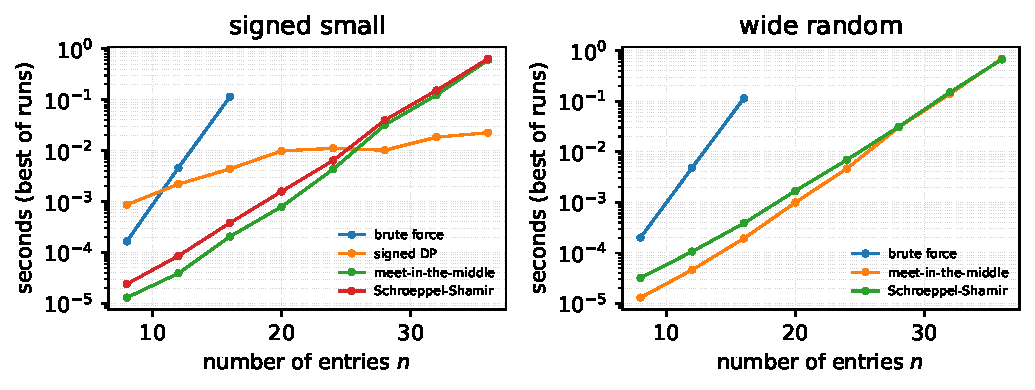
\includegraphics[width=\columnwidth]{figures/fig_runtime}
\caption{Measured runtime versus $n$ on infeasible instances, log scale. Wide
values (right) admit no pseudopolynomial table, and meet-in-the-middle and
Schroeppel--Shamir both grow exponentially; bounded values (left) are solved in
near-constant time by the signed DP.}
\label{fig:runtime}
\end{figure}

\begin{figure}[t]
\centering
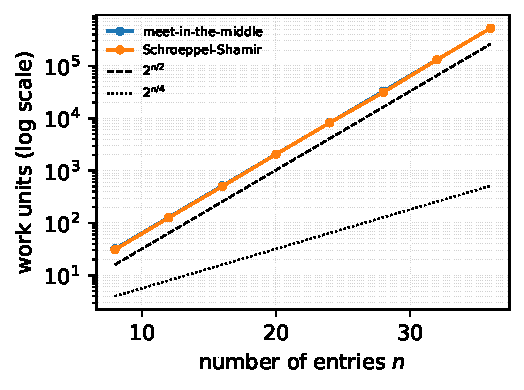
\includegraphics[width=0.86\columnwidth]{figures/fig_states}
\caption{Reported work units versus $n$ (log scale) with the reference slopes
$2^{n/2}$ and $2^{n/4}$. The measured counts track $2^{n/2}$ as predicted; the
$2^{n/4}$ line bounds the space, not the time.}
\label{fig:states}
\end{figure}

\begin{figure}[t]
\centering
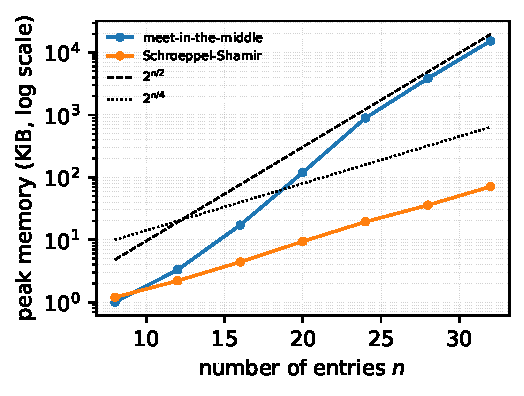
\includegraphics[width=0.86\columnwidth]{figures/fig_memory}
\caption{Peak memory versus $n$ (log scale). Meet-in-the-middle grows by about
a factor of four per four added entries ($2^{n/2}$); Schroeppel--Shamir grows
by about a factor of two ($2^{n/4}$), realizing the space saving its analysis
predicts.}
\label{fig:memory}
\end{figure}

The measurements support three observations. First, meet-in-the-middle and
Schroeppel--Shamir have the same exponential time order
($\Oh^*(2^{n/2})$); their measured times differ by a small constant factor from
the heap operations. Second, the peak-memory curves separate cleanly, matching
$2^{n/2}$ for meet-in-the-middle and $2^{n/4}$ for Schroeppel--Shamir. Third,
the signed DP is effectively linear in $n$ for bounded values and becomes the
fastest method once $n$ is large enough, but it is unusable on the wide family
because $W$ exceeds memory. Finite measurements illustrate the bounds; they do
not prove an asymptotic improvement or establish any lower bound.

\section{Formalization and Executable Artifacts}
The file \texttt{lean/SubsetSum.lean} imports only \texttt{Std} under Lean
4.19.0. It proves:
\begin{itemize}
\item \texttt{mem\_sums\_iff}: enumeration is equivalent to the inductive
selection specification;
\item \texttt{sums\_length}: the enumeration has $2^n$ entries;
\item \texttt{hasSum\_append}: the split equivalence;
\item \texttt{meetInMiddle\_correct}: executable list-based matching decides the
inductive specification;
\item \texttt{hasSum\_magnitude} and \texttt{target\_outside\_impossible}: every
feasible sum is inside the signed DP radius, and targets outside it are
impossible;
\item \texttt{restricted\_work\_bound}: the arithmetic inequality used in
Theorem~\ref{thm:restricted}.
\end{itemize}
The Lean matcher deliberately uses linear list membership; it is an executable
correctness reference, not the efficient sorted matcher. The formalization does
not verify the Python interpreter, the witness-mask implementation, the sorting
refinement, the DP table, the Schroeppel--Shamir control flow, or operational
running time. The runtime and DP correctness arguments are mathematical; the
restricted Lean theorem is an arithmetic work envelope. The general
$\Oh^*(2^{n/3})$ question is neither assumed as an axiom nor stated as a
completed theorem. All proofs compile without \texttt{sorry}, and axiom reports
are included in the source.

The Python module \texttt{src/subset\_sum.py} has no third-party dependencies.
The solvers return indices into the original sequence or \texttt{None} for
infeasibility; the empty tuple is a valid witness. Automatic selection compares
simple work estimates and makes no optimality claim. Schroeppel--Shamir is
selected explicitly because its larger constant offset is not worth paying
unless space matters.

\section{Reproduction and Validation}
From the repository root:
\begin{lstlisting}[basicstyle=\ttfamily\scriptsize,breaklines=true]
python3 -m unittest tests.test_subset_sum -v
python3 -m src.subset_sum --values 3 -2 7 0 --target 5 --method ss
python3 scripts/analysis/benchmark.py
uv run python scripts/analysis/plot_benchmarks.py   # figures + tables
cd lean && lake build
\end{lstlisting}
The unittest suite checks all lists of length zero through four over
$\{-2,0,3\}$ against all targets from $-9$ through $13$ (2{,}783 exhaustive
instances), 150 seeded random instances with up to ten entries, explicit
single-use and repeated-value cases, arbitrary-precision arithmetic, and input
validation. Every solver is compared against independent Boolean-vector
enumeration and each returned witness is checked for unique, in-range indices
and the correct sum. Passing finite tests supports implementation confidence;
it is not evidence for a general asymptotic bound. The benchmark writes CSV
tables and a provenance record under
\texttt{docs/analysis/2026-10-03/subset-sum/}; the figures and
Tables~\ref{tab:runtime}--\ref{tab:memory} are regenerated from that data.

\section{Remaining Research Goal}
To improve the worst-case bound, one must construct an algorithm with an
$\Oh^*(2^{n/3})$ upper bound for \emph{every} allowed input, justify its
arithmetic model, and account for any randomized success guarantee. Neither
favorable benchmarks nor average-case representation analyses supply that
quantifier. The recent worst-case progress for subset-balancing coefficient
sets~\cite{rw} suggests the representation technique is the most promising
direction; transferring it to the $\{0,1\}$ form remains open. This note
provides checked correctness foundations, a clean space-efficient baseline, and
reproducible measurements; the unrestricted exponent is left open.

\begin{thebibliography}{9}
\bibitem{hs} E. Horowitz and S. Sahni, ``Computing partitions with applications
to the knapsack problem,'' \emph{Journal of the ACM}, vol.~21, no.~2,
pp.~277--292, 1974.
\bibitem{ss} R. Schroeppel and A. Shamir, ``A $T=O(2^{n/2})$, $S=O(2^{n/4})$
algorithm for certain NP-complete problems,'' \emph{SIAM Journal on Computing},
vol.~10, no.~3, pp.~456--464, 1981.
\bibitem{hgj} N. Howgrave-Graham and A. Joux, ``A new generic algorithm for hard
knapsacks,'' in \emph{EUROCRYPT}, 2010.
\bibitem{bcj} A. Becker, J.-S. Coron, and A. Joux, ``Improved generic algorithms
for hard knapsacks,'' in \emph{EUROCRYPT}, 2011; IACR ePrint 2011/474.
\bibitem{chen} X. Chen, Y. Jin, T. Randolph, and R. A. Servedio, ``Subset sum
in time $2^{n/2}/\mathrm{poly}(n)$,'' in \emph{RANDOM}, 2023; arXiv:2301.07134.
\bibitem{nw} J. Nederlof and K. W\k{e}grzycki, ``Improving Schroeppel and
Shamir's algorithm for subset sum via orthogonal vectors,'' in \emph{STOC},
2021; arXiv:2010.08576.
\bibitem{rw} T. Randolph and K. W\k{e}grzycki, ``Beating meet-in-the-middle for
subset balancing problems,'' arXiv:2511.10823, 2025.
\end{thebibliography}
\end{document}
